\documentclass{article}
\usepackage[utf8]{inputenc}
\usepackage{graphicx}
\usepackage{amsmath}

\begin{document}

\section*{Confidence Intervals Short Questions}
\begin{enumerate}
    \item Given is a confidence interval \([x_1, x_2]\) of a parameter 
    \(x\) at a confidence level \(\alpha\). What is the frequentist, 
    what is the Bayesian interpretation of this interval?
    \begin{itemize}
        \item \textit{Frequentist Interpretation:}
        \begin{itemize} 
            \item If the same experiment is repeated many times, $\alpha$ of the constructed confidence intervals will contain the true parameter value.
        \end{itemize}
        \item \textit{Bayesian Interpretation:}
        \begin{itemize}
            \item Confidence Intervals are credibility intervals. 
            \item Credibility intervals contain the true parameter with a 
            probability \(\alpha\), based on the posterior probability density 
            function (PDF).
        \end{itemize} 
    \end{itemize}
    \item What role does the prior in Bayesian statistics play?
    \begin{itemize}
        \item The prior represents the initial assumptions about the 
        parameter before observing the data.
        \item The choice of the prior can significantly impact the resulting 
        credibility interval.
    \end{itemize}
    \item What freedom is there in choosing these intervals?
    \begin{itemize}
        \item One can choose:
        \begin{itemize}
            \item symmetric interval around the expectation $x_+-\mu=\mu-x_-$ 
            \item shortest interval, minimizing $x_+-x_-$
            \item central interval given by 
            $\int_{-\infty}^{x_-}P(x)\,\text{d}x=\int_{x_+}^{\infty}P(x)\,\text{d}x =\frac{1-\alpha}{2}$
        \end{itemize}
    \end{itemize}
    \item What happens in the special case of symmetrical PDF?
    \begin{itemize}
        \item For symmetric PDFs, all these intervals are equivalent.
    \end{itemize}
    \item What is the difference between intervals and upper/lower limits?
    \begin{itemize}
        \item \textit{Confidence Intervals}
        \begin{itemize}
            \item Provide a range within which the parameter is believed to lie with a certain confidence level.
            \item Example: A 95\% confidence interval means there is a 95\% probability that the interval contains the true parameter value.
        \end{itemize}
        \item \textit{Upper/Lower Limits}
        \begin{itemize}
            \item Indicate bounds above or below which the parameter lies with a certain confidence level.
            \item Example: A 95\% upper limit means there is a 95\% probability that the true parameter value is below this limit.
        \end{itemize}
    \end{itemize}
\end{enumerate}

\begin{figure}
    \centering
    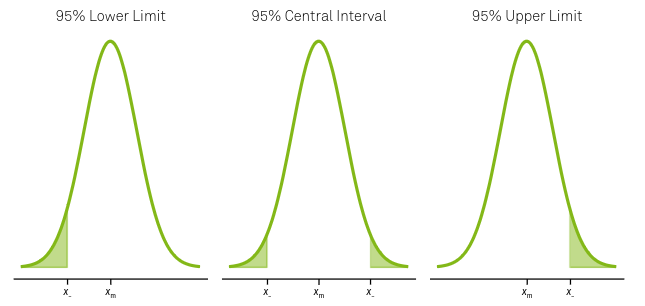
\includegraphics[width=\textwidth]{plot.png}
    \label{fig:plot}
\end{figure}

\end{document}
